% SPDX-License-Identifier: Apache-2.0
\section{Background}
\label{sec:background}

\subsection{The YubiKey's USB interfaces}

A YubiKey 5 shows three USB interfaces to the host~\cite{yk-usb}
(verified). Table~\ref{tab:interfaces} lists them. Each interface is a
separate unit for the host's drivers. A process can claim one interface and
leave the others to other drivers.

\begin{table}[t]
\centering
\caption{YubiKey 5 USB interfaces}
\label{tab:interfaces}
\scriptsize
\begin{tabular}{@{}l>{\raggedright\arraybackslash}p{17mm}>{\raggedright\arraybackslash}p{15mm}>{\raggedright\arraybackslash}p{23mm}@{}}
\toprule
Interface & Class & Endpoints & Functions \\
\midrule
OTP & HID keyboard & interrupt IN & Yubico OTP, static password \\
FIDO & HID, usage page 0xF1D0 & interrupt IN and OUT & U2F, FIDO2 \\
CCID & smart card & bulk IN and OUT & PIV, OpenPGP, OATH \\
\bottomrule
\end{tabular}
\end{table}

The goals of Section~\ref{sec:intro} map onto the interfaces. WebAuthn needs
only the FIDO interface. OpenPGP and PIV need the CCID interface. The OTP
interface is not a goal.

\subsection{CTAPHID}

A FIDO key on USB talks CTAPHID~\cite{ctap21}. CTAPHID cuts each message into
64-byte HID reports. Figure~\ref{fig:packets} shows the two packet kinds. The
first packet holds the channel ID (CID), the command, and the payload length.
Each continuation packet holds the CID and a sequence number. One message can
hold up to 7609 bytes: 57 bytes in the first packet and 59 bytes in each of
128 continuation packets.

\begin{figure}[t]
\centering
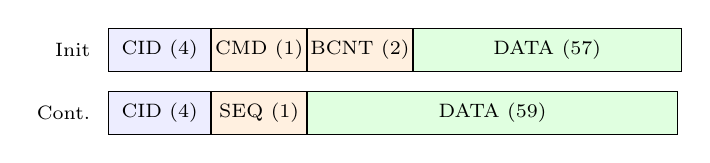
\begin{tikzpicture}[font=\scriptsize]
  \tikzset{fld/.style={draw,minimum height=5.5mm,inner sep=1pt,anchor=west}}
  \node[anchor=east] at (-1mm,0) {Init};
  \node[fld,fill=blue!7,minimum width=13mm] (a) at (0,0) {CID (4)};
  \node[fld,fill=orange!12,minimum width=12mm] (b) at (a.east) {CMD (1)};
  \node[fld,fill=orange!12,minimum width=13mm] (c) at (b.east) {BCNT (2)};
  \node[fld,fill=green!12,minimum width=34mm] at (c.east) {DATA (57)};
  \node[anchor=east] at (-1mm,-8mm) {Cont.};
  \node[fld,fill=blue!7,minimum width=13mm] (d) at (0,-8mm) {CID (4)};
  \node[fld,fill=orange!12,minimum width=12mm] (e) at (d.east) {SEQ (1)};
  \node[fld,fill=green!12,minimum width=47mm] at (e.east) {DATA (59)};
\end{tikzpicture}
\caption{The two CTAPHID packet kinds. Each is one 64-byte HID report. Field
sizes are in bytes; the boxes are not to scale. In an init packet, bit 7 of
CMD is set.}
\label{fig:packets}
\end{figure}

A client first sends \code{CTAPHID\_INIT} on the broadcast channel
\code{0xFFFFFFFF} with an 8-byte nonce. The key replies with a new channel
ID. All later messages use that channel. FIDO2 requests travel as
\code{CTAPHID\_CBOR} messages. The first payload byte names the CTAP2
command. For example, \code{0x02} is \code{getAssertion} and \code{0x07} is
\code{reset}.

While the key waits for a touch, it sends \code{CTAPHID\_KEEPALIVE} at least
every 100\,ms~\cite{ctap21} (verified). Chrome on Linux waits 20\,s for a
FIDO device, and each keepalive starts that wait again~\cite{chromefido}
(verified). A relay that passes keepalives through therefore has no hard
time limit for the touch.

\subsection{Linux devices for HID}

On a normal Linux host the kernel driver \code{usbhid} binds to each HID
interface. It creates one \code{/dev/hidrawN} node per interface. Chrome,
libfido2, and OpenSSH all find FIDO keys through these nodes. Chrome uses any
HID device that declares usage page \code{0xF1D0}, on any bus~\cite{chromefido}
(verified).

The kernel module \code{uhid} lets a userspace process create a HID device.
The process writes a report descriptor to \code{/dev/uhid}. The kernel then
creates a new \code{hidraw} node for it. A relay can use this to make a
\term{virtual} FIDO key on the remote host.

Below \code{hidraw} is \term{usbfs}: one node per USB device under
\code{/dev/bus/usb}. A process that opens it can read the descriptors, detach
the kernel driver from an interface, claim the interface, and run transfers
with \code{ioctl} calls. libusb uses usbfs on Linux.
